% PAKDD submission (Springer LNCS). Main paper only; the appendices of
% steerf.tex are paper/pakdd_supp.tex, submitted as supplementary material.
% Every measured number is a \num{} slot filled from results/*.tex, exactly as
% in steerf.tex: no number in this file is typed by hand.
\documentclass[runningheads]{llncs}
\usepackage[T1]{fontenc}
\usepackage{lmodern}
\usepackage[utf8]{inputenc}
\usepackage{microtype}
\usepackage{graphicx}
\usepackage{amsmath}
\usepackage{amssymb}
\usepackage{booktabs}
\usepackage{xcolor}
\usepackage{tikz}
\usepackage[hidelinks]{hyperref}

% ---- macros -----------------------------------------------------------
\newcommand{\Htraj}{\mathcal{H}}
\newcommand{\Htogo}{H_{\mathrm{togo}}}
\newcommand{\AH}{A_{H}}
\newcommand{\Om}{\Omega}
\newcommand{\E}{\mathbb{E}}
\newcommand{\gradt}{\nabla_{\theta}}
\newcommand{\pit}{\pi_{\theta}}

% ---- generated numbers (see steerf.tex for the rationale) --------------
\providecommand{\PENDING}{\textcolor{red}{\textbf{--}}}
\newcommand{\num}[1]{\ifcsname #1\endcsname\csname #1\endcsname\else\PENDING\fi}
\newcommand{\loadnumbers}[1]{%
  \IfFileExists{../results/#1}{\input{../results/#1}}{%
    \IfFileExists{results/#1}{\input{results/#1}}{}}}
\loadnumbers{numbers.tex}
\loadnumbers{numbers-locality.tex}
\loadnumbers{numbers-decomp.tex}

\begin{document}
\title{Where Does Entropy Collapse Go?\\
Measuring the Visitation Channel That Token-Level Entropy Control Misses}
\titlerunning{Where Does Entropy Collapse Go?}
\author{Anonymous Authors}
\authorrunning{Anonymous}
\institute{Anonymous Institution}
\maketitle

\begin{abstract}
Reinforcement learning with verifiable rewards (RLVR) drives a language model's
entropy toward zero, and the standard remedies act token by token. We ask where the
lost entropy goes. The change in trajectory entropy splits exactly into a
\emph{local} channel, sharpening at the states the policy visits, and a
\emph{visitation} channel, a change in which states it visits; token-level control
acts only on the first. Measured between checkpoints of a $1.5$B model,
$\num{DecGrpoShare}$ of the entropy GRPO loses by step $100$ goes through the
visitation channel, and a registered replication on two further seeds gives
$\num{DecRepGrpoShare}$ and $\num{DecRepSignedShare}$. In the run we followed, most of
the loss occurs within the first $50$ steps. We show why the local channel cannot be
extended to cover the other, and derive the visitation term as a per-token advantage
that sums to zero over sibling rollouts, so aggregate entropy cannot register it. A
five-arm experiment over three paired seeds bears this out: changing the damping
mechanism moves aggregate entropy, changing only the visitation signal barely does.
We make no accuracy claim; the paper is an account of where entropy collapse happens
and of what aggregate entropy curves cannot show.
\keywords{Large language models \and Reinforcement learning \and Entropy collapse
\and Reasoning \and Analysis}
\end{abstract}

% =====================================================================
\section{Introduction}
\label{sec:intro}

Policy-gradient fine-tuning with verifiable rewards sharpens a language model's output
distribution. Measured as the mean per-token entropy, the sharpening is fast, monotone
and, past a point, coincident with the end of useful learning. The standard remedies
spend part of the update budget slowing it down: an entropy bonus, a KL anchor, a clip
on the tokens that lose most entropy, or a per-token re-weighting of the policy loss by
a first-order estimate of the entropy each token's update destroys~\cite{steer}. All of
them act on the conditional distribution at a state the policy has reached. This paper
asks a prior question: when RLVR loses entropy, how much of the loss is sharpening at
the states the policy visits, and how much is a change in which states it visits?

The distinction matters because token-level control can see only the first, and the
omission is structural. Fig.~\ref{fig:branch} shows the case. At a state with two
equiprobable continuations the conditional distribution is as entropic as it can be,
and its first-order entropy change under a small push is zero. Yet shifting mass from
a continuation that leads into a rich sub-tree to one that leads into a dead end
removes all the downstream diversity the first carried. The branch is locally safe;
which branch is visited is not.

\begin{figure}[t]
\centering
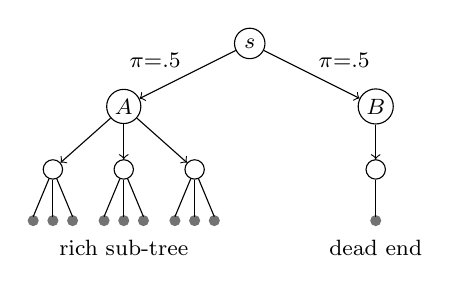
\begin{tikzpicture}[
  every node/.style={font=\footnotesize},
  st/.style={circle, draw, inner sep=1.4pt, minimum size=11pt},
  sm/.style={circle, draw, minimum size=7pt, inner sep=0pt},
  lf/.style={circle, fill=black!55, inner sep=0pt, minimum size=4pt}]
\node[st] (s) at (0,0) {$s$};
\node[st] (a) at (-1.6,-0.8) {$A$};
\node[st] (b) at (1.6,-0.8) {$B$};
\draw[->] (s) -- node[above left=-1pt] {$\pi{=}.5$} (a);
\draw[->] (s) -- node[above right=-1pt] {$\pi{=}.5$} (b);
\foreach \i/\x in {1/-2.5, 2/-1.6, 3/-0.7} {
  \node[sm] (m\i) at (\x,-1.6) {};
  \draw[->] (a) -- (m\i);
  \foreach \d in {-0.25, 0, 0.25} {
    \node[lf] at (\x+\d,-2.25) {};
    \draw (m\i) -- (\x+\d,-2.2);
  }
}
\node[sm] (bb) at (1.6,-1.6) {};
\draw[->] (b) -- (bb);
\node[lf] at (1.6,-2.25) {};
\draw (bb) -- (1.6,-2.2);
\node at (-1.6,-2.6) {rich sub-tree};
\node at (1.6,-2.6) {dead end};
\end{tikzpicture}
\caption{At $s$ the conditional entropy is maximal and its first-order change is $0$
(local channel), yet moving mass from $A$ to $B$ removes $A$'s downstream diversity
(visitation channel). Token-level entropy control sees only the first.}
\label{fig:branch}
\end{figure}

Writing $\Htraj(\pit \mid x)$ for the entropy of the distribution over whole
responses, its gradient splits, by the product rule and with no approximation, into a
\emph{local} term that holds visited states fixed --- what a per-token estimate
measures --- and a \emph{visitation} term that differentiates the probability of
reaching each state. The local estimate vanishes at a flat branch point, correctly,
since the entropy loss there is second order; the visitation term's prefactor is
largest at those same points.

How much of real collapse goes through each channel is an empirical question, and the
same split answers it exactly between two checkpoints. From the base model to step
$100$ of GRPO, $\num{DecGrpoShare}$ of the lost trajectory entropy goes through
visitation, and the share replicates on two other seeds (Section~\ref{sec:decomp}).
Most of what is called entropy collapse is therefore not sharpening at fixed states but
the policy settling on paths along which the base model was already confident --- the
part token-level control does not touch. Within the scope of what we measured, this has
three practical consequences. First, finer per-token weights are the wrong lever: the
two damping variants we tested leave the split where GRPO puts it, so preserving
diversity calls for objectives that act on which paths are sampled and reinforced,
such as outcome-level exploration~\cite{song2025outcome} or rollouts that diversify
prefixes~\cite{cao2026treeadv}. Second, timing matters: by step $50$ the run we
followed had already lost $\num{DecSecSignedADH}$ of the $\num{DecSignedDH}$ nats it
lost by step $100$, so an intervention switched on once entropy looks low arrives after
most of the collapse. Third, mean token entropy is the wrong monitor: it cannot
register a change in which paths are visited (Section~\ref{sec:zerosum}), whereas the
split needs only samples and forward passes at two checkpoints.

Our contributions are:
\begin{itemize}
\item \textbf{A measurement of where collapse goes}: an exact between-checkpoint split
      of the entropy that training loses, which assigns $\num{DecGrpoShare}$ of GRPO's
      loss to the visitation channel, replicated on two further seeds
      (Section~\ref{sec:decomp}).
\item \textbf{Why token-level control cannot reach it}: the local estimator vanishes
      at flat branch points, where the visitation prefactor is largest
      (Section~\ref{sec:channels}).
\item \textbf{An estimable visitation term and its diagnostic consequence}: a per-token
      advantage $\AH$ that sums to zero over siblings, so aggregate token entropy
      cannot diagnose it (Section~\ref{sec:ahdef}).
\item \textbf{A test of that consequence}: five arms that separate the damping
      mechanism from the visitation signal (Section~\ref{sec:dissoc}).
\end{itemize}

% =====================================================================
\section{Background and Related Work}
\label{sec:prelim}

A prompt is $x$, a response $y = y_{1:T}$, and $s_t = (x, y_{<t})$ the state before
token $t$. GRPO~\cite{shao2024deepseekmath} samples $n$ responses per prompt and
broadcasts the group-standardized reward to every token.

\paragraph{Entropy collapse and its control.} Entropy decay under policy-gradient
fine-tuning of reasoning models is tied to the stall of improvement~\cite{cui2025bentropy}
and is countered by an asymmetric clip~\cite{yu2025dapo}, by restricting updates on
high-covariance tokens~\cite{cui2025bentropy}, by KL control with reference
resets~\cite{liu2025bprorl}, or by selective entropy regularization, since a naive bonus
tends to explode~\cite{rethinkingentropyreg}. Training on a minority of high-entropy
``forking'' tokens suffices~\cite{wang2025dbeyond}, and several schemes shape advantages
or rewards with token entropy~\cite{cheng2025reasoning,tan2025gtpo,zhang2025dedge}.
STEER~\cite{steer} multiplies each token's surrogate loss by a weight in
$[\lambda_{\min}, 1]$ derived from a first-order estimate $\Om$ of the change in
conditional entropy at a fixed state. All of these act on conditional distributions at
visited states, that is, on the local channel.

\paragraph{Trajectory-level diversity.} Token-level entropy can stay high while the
diversity of final answers falls~\cite{wu2025ainvisible}, and outcome-level exploration
targets that diversity directly~\cite{song2025outcome}. The visitation channel is a
mechanism for the first observation. Tree-structured rollouts give intermediate
decisions their own reward credit~\cite{hou2025treerl,yang2025treerpo,cao2026treeadv}
and choose where to branch~\cite{cao2026treeadv,khomich2026epig}; we use the same
structure to supply a baseline for remaining entropy rather than for reward. The
identity we rest on is the entropy term of the maximum-entropy RL objective, whose
policy gradient is standard there~\cite{schulman2017equivalence,levine2018reinforcement};
what we add is its use to measure real collapse and to locate token-level control.

% =====================================================================
\section{Two Channels}
\label{sec:channels}

The autoregressive factorization gives $\Htraj(\pit \mid x) = \E_{y \sim
\pit}[\sum_t H(\pit(\cdot \mid s_t))]$. Both the integrand and the measure depend on
$\theta$; with $f_\theta(y) := \sum_t H(\pit(\cdot \mid s_t(y)))$, the product rule and
the score-function identity give, with no approximation,
\begin{equation}
\gradt \Htraj
= \underbrace{\E\bigl[\gradt f_\theta(y)\bigr]}_{(\mathrm{L})\ \text{local}}
+ \underbrace{\E\bigl[f_\theta(y)\,\gradt \log \pit(y \mid x)\bigr]}_{(\mathrm{V})\ \text{visitation}}.
\label{eq:twochannel}
\end{equation}
(L) holds the visited states fixed and is what $\Om$ estimates. (V) holds per-state
entropies fixed and asks how the probability of reaching each state changes. The two can
have opposite signs, so driving (L) to zero does not bound $\gradt \Htraj$.

\paragraph{The local channel cannot be repaired.} One might expect the channels to
coincide, since branch points are uncertain positions. Three facts rule this out.
(i)~$\Om \propto \pi_a(1-\pi_a)(H - I_a)$ with $I_a = -\log \pit(a \mid s)$ and
$H = \E[I_a]$, so $|\Om|$ is set by the spread of surprisal, not the level of entropy.
(ii)~At a uniform branch point $I_a = H$ for every $a$, so $\Om \equiv 0$.
(iii)~That zero is correct: the logit derivative of the conditional entropy,
$-\pit(a)(\log \pit(a) + H)$, vanishes at a uniform distribution, so the local loss is
entirely second order. The visitation prefactor, in contrast, is $1 - \pi_a$, which
tends to $1$ as the distribution flattens --- exactly where a group of samples is
certain to diverge. The local signal vanishes where the visitation prefactor is largest,
so no refinement of the local term recovers what it omits. Table~\ref{tab:anticorr}
evaluates both on a family of distributions from confident to flat; full derivations
are in the supplementary material.

\begin{table}[t]
\caption{The two channels are oppositely ordered around flat branch points. The top
token has mass $q$, the rest is spread uniformly over $m$ tokens; $P(\mathrm{split})$
is the probability that $n{=}8$ samples do not all agree.}
\label{tab:anticorr}
\centering
\setlength{\tabcolsep}{6pt}
\begin{tabular}{@{}lcccc@{}}
\toprule
distribution & $H$ & $P(\mathrm{split})$ & $\E|\Om|/|A|$ & $\E[1{-}\pi_a]$ \\
\midrule
$q{=}.99$          & 0.10 & 0.08 & 0.092 & 0.020 \\
$q{=}.9$, tail     & 1.25 & 0.57 & \textbf{1.129} & 0.190 \\
$q{=}.6$, $m{=}3$  & 1.11 & 0.98 & 0.457 & 0.587 \\
uniform, $k{=}10$  & 2.30 & \textbf{1.00} & \textbf{0.000} & \textbf{0.900} \\
uniform, $k{=}100$ & 4.61 & \textbf{1.00} & \textbf{0.000} & \textbf{0.990} \\
\bottomrule
\end{tabular}
\end{table}

% =====================================================================
\section{Where Measured Collapse Goes}
\label{sec:decomp}

Equation~\eqref{eq:twochannel} splits a gradient; between two checkpoints $a$ and $b$
the change itself splits the same way. With $\E_x[S_m]$ the mean, over responses
sampled from $x$, of model $m$'s next-token entropies summed along the response,
\begin{equation}
\Delta H = \underbrace{\E_b[S_b] - \E_b[S_a]}_{L}
         + \underbrace{\E_b[S_a] - \E_a[S_a]}_{V},
\label{eq:split}
\end{equation}
exactly. $L$ is the change at the states $b$ visits; $V$ is the change in which states
are visited, scored by one fixed model. The split depends on whose states are used, so
we average it with the reverse ordering ($L' = \E_a[S_b] - \E_a[S_a]$,
$V' = \E_b[S_b] - \E_a[S_b]$), which also adds to $\Delta H$ exactly.

\paragraph{Procedure.} We use $\num{DecNprompts}$ training prompts of DAPO-Math-17k,
the same for every checkpoint, and four responses per prompt sampled at temperature
$1$, top-$p$ $1$, up to $3072$ tokens --- the training sampler. Every response set of an
interval is scored by both of its checkpoints with the full-vocabulary next-token
entropy from an fp32 softmax. Intervals are 95\% percentile bootstraps over prompts
($10{,}000$ resamples), paired across checkpoints. Two rules were registered before any
sample was drawn: a measurable visitation share is claimed only if the interval of $V$
excludes zero with the sign of $\Delta H$; and a damping arm is called consistent with
acting on the local channel only if its difference from GRPO in $L$ excludes zero and
exceeds its difference in $V$. A replication on other seeds was registered after the
seed-$1$ result and before its samples; it uses the two retained checkpoints off seed
$1$ that match a primary arm.

\begin{table}[t]
\caption{Where the trajectory entropy lost between the base model
($H_a = \num{DecGrpoHa}$ nats per response) and a later checkpoint goes, in nats per
response. $L$: same states, sharper conditionals; $V$: other states visited;
$\Delta H = L + V$ exactly. Brackets: 95\% prompt-bootstrap interval.}
\label{tab:decomp}
\centering
\setlength{\tabcolsep}{5pt}
\begin{tabular}{@{}lrrrc@{}}
\toprule
base $\to$ & $\Delta H$ & $L$ & $V$ & $V/\Delta H$ \\
\midrule
\multicolumn{5}{@{}l}{\emph{seed $1$, step $100$}} \\
GRPO & $\num{DecGrpoDH}$ & $\num{DecGrpoL}$ & $\num{DecGrpoV}$ & \num{DecGrpoShare} [\num{DecGrpoShareLo}, \num{DecGrpoShareHi}] \\
\textsc{permuted} & $\num{DecPermDH}$ & $\num{DecPermL}$ & $\num{DecPermV}$ & \num{DecPermShare} [\num{DecPermShareLo}, \num{DecPermShareHi}] \\
\textsc{signed} & $\num{DecSignedDH}$ & $\num{DecSignedL}$ & $\num{DecSignedV}$ & \num{DecSignedShare} [\num{DecSignedShareLo}, \num{DecSignedShareHi}] \\
\midrule
\multicolumn{5}{@{}l}{\emph{replication, other seeds}} \\
GRPO, seed $2$, step $80$ & $\num{DecRepGrpoDH}$ & $\num{DecRepGrpoL}$ & $\num{DecRepGrpoV}$ & \num{DecRepGrpoShare} [\num{DecRepGrpoShareLo}, \num{DecRepGrpoShareHi}] \\
\textsc{signed}, seed $3$, step $100$ & $\num{DecRepSignedDH}$ & $\num{DecRepSignedL}$ & $\num{DecRepSignedV}$ & \num{DecRepSignedShare} [\num{DecRepSignedShareLo}, \num{DecRepSignedShareHi}] \\
\bottomrule
\end{tabular}
\end{table}

\begin{table}[t]
\caption{Secondary intervals, seed $1$, registered without a decision rule; nats per
response. The \textsc{signed} rows come from a $200$-step re-run of that arm.}
\label{tab:decompsec}
\centering
\setlength{\tabcolsep}{5pt}
\begin{tabular}{@{}lrrrc@{}}
\toprule
interval & $\Delta H$ & $L$ & $V$ & $V/\Delta H$ \\
\midrule
\textsc{signed} $0 \to 50$ & $\num{DecSecSignedADH}$ & $\num{DecSecSignedAL}$ & $\num{DecSecSignedAV}$ & \num{DecSecSignedAShare} [\num{DecSecSignedAShareLo}, \num{DecSecSignedAShareHi}] \\
\textsc{signed} $50 \to 100$ & $\num{DecSecSignedBDH}$ & $\num{DecSecSignedBL}$ & $\num{DecSecSignedBV}$ & \num{DecSecSignedBShare} [\num{DecSecSignedBShareLo}, \num{DecSecSignedBShareHi}] \\
\textsc{signed} $100 \to 150$ & $\num{DecSecSignedCDH}$ & $\num{DecSecSignedCL}$ & $\num{DecSecSignedCV}$ & \num{DecSecSignedCShare} [\num{DecSecSignedCShareLo}, \num{DecSecSignedCShareHi}] \\
\textsc{signed} $150 \to 200$ & $\num{DecSecSignedDDH}$ & $\num{DecSecSignedDL}$ & $\num{DecSecSignedDV}$ & \num{DecSecSignedDShare} [\num{DecSecSignedDShareLo}, \num{DecSecSignedDShareHi}] \\
GRPO $80 \to 110$ & $\num{DecSecGrpoLateDH}$ & $\num{DecSecGrpoLateL}$ & $\num{DecSecGrpoLateV}$ & \num{DecSecGrpoLateShare} [\num{DecSecGrpoLateShareLo}, \num{DecSecGrpoLateShareHi}] \\
\textsc{permuted} $80 \to 110$ & $\num{DecSecPermLateDH}$ & $\num{DecSecPermLateL}$ & $\num{DecSecPermLateV}$ & \num{DecSecPermLateShare} [\num{DecSecPermLateShareLo}, \num{DecSecPermLateShareHi}] \\
\bottomrule
\end{tabular}
\end{table}

\paragraph{Result.} GRPO loses $\num{DecGrpoDH}$ nats per response, and the visitation
channel carries $\num{DecGrpoShare}$ of it, which meets the registered criterion
(Table~\ref{tab:decomp}). The replication meets the same criterion: GRPO on seed $2$
gives $\num{DecRepGrpoShare}$ and the campaign's \textsc{signed} run on seed $3$ gives
$\num{DecRepSignedShare}$. Most of the measured collapse is therefore not sharpening at
the states the policy already visited: the trained policy moves to states where the
base model was already confident, and the local channel, the only one a token-level
estimator sees, carries the remainder. The two damping arms (Section~\ref{sec:dissoc})
give nearly the same split as GRPO.

\paragraph{Timing.} The loss is front-loaded (Table~\ref{tab:decompsec}): by step $50$
the \textsc{signed} run has already lost $\num{DecSecSignedADH}$ nats,
$\num{DecSecSignedAShare}$ of it through visitation. Between later checkpoints the
changes are much smaller and the local channel's part is larger (visitation share
$\num{DecSecSignedBShare}$ from step $50$ to $100$), and where entropy rises late the
rise again goes mostly through visitation.

\paragraph{Checks.} Because $\Htraj$ grows with response length and long responses are
cut at $3072$ tokens, we checked, after seeing the result, whether truncation or length
carries the share: without truncated responses, per token, or both, it stays between
$\num{DecRobustMin}$ and $\num{DecRobustMax}$ on seed $1$ and between
$\num{DecRepRobustMin}$ and $\num{DecRepRobustMax}$ on the replication (exploratory).
The second registered prediction is not borne out: relative to GRPO the damping arms
change $V$ more than $L$ (\textsc{permuted} $\num{DecPermdV}$ against
$\num{DecPermdL}$, \textsc{signed} $\num{DecSigneddV}$ against $\num{DecSigneddL}$
nats), so the difference damping makes, integrated over training, is also mostly a
difference in where the policy goes.

% =====================================================================
\section{Why Aggregate Entropy Cannot See It}
\label{sec:ahdef}

\paragraph{The visitation term as an advantage.} Expanding (V) into a double sum over
the position $t$ of an entropy and the position $u$ of a score, every term with
$u \ge t$ vanishes by causality, leaving a REINFORCE estimator whose reward-to-go is the
remaining conditional entropy,
\begin{equation}
(\mathrm{V}) = \E\Bigl[\textstyle\sum_u \gradt \log \pit(y_u \mid s_u)\,
\Htogo(s_u \oplus y_u)\Bigr],
\label{eq:togo}
\end{equation}
with $\Htogo(s_u \oplus y_u) := \sum_{t > u} H(\pit(\cdot \mid s_t))$. Any function of $s_u$ alone is an admissible baseline. We use the mean of $\Htogo$ over
rollouts in the group whose prefixes $y_{<u}$ agree exactly, giving the advantage
$\AH(s_u, y_u) := \Htogo(s_u \oplus y_u) - \bar{H}_{\mathrm{togo}}(s_u)$, non-zero only
where siblings share a prefix and then diverge. Independent samples almost never share
prefixes, so we schedule the sharing with a fixed tree (a root cut at depths
$\{64, 192, 384\}$ with branching factor $2$, $n = 8$ leaves), used only as a device
for the estimator. With $n$ leaves at most $n-1$ nodes branch, so at most $2(n-1)/T$ of
positions carry $\AH \ne 0$ under any sampler.

\paragraph{The correction cannot move the mean.}
\label{sec:zerosum}
On each sibling set $\sum_j \AH(s_u, y^{(j)}_u) = 0$. A correction built on $\AH$ can
therefore change which sibling is damped but not how much damping there is on
average, and an average over all response tokens should barely register it: aggregate
token entropy is not a diagnostic for whether the visitation channel is acted on. We
turn $\AH$ into a bounded adjustment of STEER's token weight, forecasting $\Htogo$ with
two multi-token-prediction heads (details in the supplementary material). The
correction is an instrument for testing this prediction, not a proposed training
method.

\subsection{A test: aggregate entropy tracks the mechanism, not the signal}
\label{sec:dissoc}

\paragraph{Setup.} All runs fine-tune Qwen2.5-Math-1.5B~\cite{yang2024aqwen} on
DAPO-Math-17k~\cite{yu2025dapo} for $110$ steps of $512$ prompts with GRPO ($n = 8$,
learning rate $10^{-6}$, responses up to $3072$ tokens, clip $0.2/0.28$, no entropy
bonus or KL). Five arms separate the \emph{damping mechanism} (tree sampler, support,
token-weight damping) from the \emph{signal} $\AH$: GRPO; \textsc{steer} (local $\Om$
only); \textsc{uniform}, which damps every supported position equally and so removes
the signal while keeping its support; \textsc{permuted}, which shuffles $\AH$ within
each sibling set, keeping magnitudes and the zero sum but destroying the branch--score
assignment; and \textsc{signed}, the correction as derived (Table~\ref{tab:arms}).
Every run validates on AIME24 ($30$ problems, $32$ samples) every $10$ steps; one
evaluation has an across-problem standard error of $\num{SEaime}$. Each run is reduced
to its mean over steps $40$--$110$, arms are paired within a seed, and contrasts use a
paired $t$ over the $\num{Nseedsused}$ seeds on which all arms finished
($\num{Seedset}$). The plan was registered before the runs.

\begin{table}[t]
\caption{The five arms. \textsc{uniform} and \textsc{permuted} keep the damping
mechanism and remove the branch-specific $\AH$ signal in two different ways.}
\label{tab:arms}
\centering
\setlength{\tabcolsep}{6pt}
\begin{tabular}{@{}llll@{}}
\toprule
arm & rollout & token weight & signal in the weight \\
\midrule
GRPO              & plain & none           & none \\
\textsc{steer}    & plain & local $\Om$    & none \\
\textsc{uniform}  & tree  & $\Om$ + damping & support only \\
\textsc{permuted} & tree  & $\Om$ + damping & $\AH$ shuffled within siblings \\
\textsc{signed}   & tree  & $\Om$ + damping & $\AH$ as derived \\
\bottomrule
\end{tabular}
\end{table}

\begin{table}[t]
\caption{Converged token-mean entropy, trajectory entropy $\Htraj$ (nats per response)
and AIME24 acc@32, paired within a seed ($\mathrm{df} = n-1$), grouped by what each
contrast changes.}
\label{tab:entropy}
\centering
\setlength{\tabcolsep}{3.5pt}
\begin{tabular}{@{}lrrrrrrr@{}}
\toprule
contrast & $n$ & $\Delta$ent. & $t$ & $\Delta\Htraj$ & $t$ & $\Delta$acc & $t$ \\
\midrule
\multicolumn{8}{@{}l}{\emph{the damping mechanism changes, the $\AH$ signal does not}} \\
\textsc{steer} $-$ GRPO & \num{Nsteergrpo} & $\num{Csteergrpoentropy}$ & $\num{Tsteergrpoentropy}$ & $\num{Csteergrpohtraj}$ & $\num{Tsteergrpohtraj}$ & $\num{Csteergrpoacc}$ & $\num{Tsteergrpoacc}$ \\
\textsc{unif} $-$ \textsc{steer} & \num{Nuniformsteer} & $\num{Cuniformsteerentropy}$ & $\num{Tuniformsteerentropy}$ & $\num{Cuniformsteerhtraj}$ & $\num{Tuniformsteerhtraj}$ & $\num{Cuniformsteeracc}$ & $\num{Tuniformsteeracc}$ \\
\midrule
\multicolumn{8}{@{}l}{\emph{the $\AH$ signal changes, the damping mechanism does not}} \\
\textsc{signed} $-$ \textsc{unif} & \num{Nsigneduniform} & $\num{Csigneduniformentropy}$ & $\num{Tsigneduniformentropy}$ & $\num{Csigneduniformhtraj}$ & $\num{Tsigneduniformhtraj}$ & $\num{Csigneduniformacc}$ & $\num{Tsigneduniformacc}$ \\
\textsc{signed} $-$ \textsc{perm} & \num{Nsignedpermuted} & $\num{Csignedpermutedentropy}$ & $\num{Tsignedpermutedentropy}$ & $\num{Csignedpermutedhtraj}$ & $\num{Tsignedpermutedhtraj}$ & $\num{Csignedpermutedacc}$ & $\num{Tsignedpermutedacc}$ \\
\bottomrule
\end{tabular}
\end{table}

\paragraph{Result.} Across all three paired seeds, changing the damping mechanism
shifts aggregate entropy far more than changing the signal with the mechanism held
fixed (Table~\ref{tab:entropy}): turning the damping on shifts it by
$\num{Csteergrpoentropy}$ and adding the tree with uniform damping by
$\num{Cuniformsteerentropy}$, whereas removing the signal shifts it by
$\num{Csigneduniformentropy}$ and destroying the branch--score assignment by
$\num{Csignedpermutedentropy}$. The split survives length correction: on $\Htraj$ the
mechanism contrasts are $\num{Csteergrpohtraj}$ and $\num{Cuniformsteerhtraj}$ nats per
response and the signal contrasts $\num{Csigneduniformhtraj}$ and
$\num{Csignedpermutedhtraj}$. Aggregate entropy reflects the damping mechanism, not the
visitation signal, which is the dissociation the zero sum predicts. Three seeds
establish the pattern more firmly than its effect sizes; the positive prediction, that
the spread across siblings widens, is not measured.

\paragraph{Accuracy.} The registered accuracy test, \textsc{signed} $-$
\textsc{uniform}, straddles zero across seeds ($\num{CLosigneduniformacc}$ to
$\num{CHisigneduniformacc}$), and the gaps between arms are smaller than GRPO's own
spread across seeds, $\num{Sgrpoacc}$, so we make no accuracy claim. Per-arm results,
ablations and the full registration are in the supplementary material.

% =====================================================================
\section{Limitations and Conclusion}
\label{sec:conclusion}

\paragraph{Limitations.} Every result is on one $1.5$B mathematics model. The
decomposition rests on seed $1$ and one retained checkpoint each of seeds $2$ and $3$,
so the seed-$2$ point is at step $80$; it measures the split between checkpoints, not
the gradient's, and the seed-$1$ \textsc{signed} checkpoint is a re-run of that
configuration on different hardware. The dissociation uses three seeds and AIME24's
$30$ problems for validation. The local--visitation trade-off at real branch points is
derived, not measured, and the $\AH$ estimator rests on an approximation inherited from
STEER (an update changes only the sampled logit) that is false for shared parameters.

\paragraph{Conclusion.} Entropy collapse in RLVR is mostly a change in where the policy
goes. Measured between checkpoints, $\num{DecGrpoShare}$ of the trajectory entropy GRPO
loses goes through the visitation channel, a share that replicates on two further
seeds, and token-level entropy control acts only on the remainder. The local estimator
vanishes, for a correct reason, exactly where the visitation term is largest; the
visitation term is estimable but sums to zero over siblings, so aggregate entropy
cannot register it, and the experiment observes that dissociation. Whether the share
holds across model scales, and which path-level objectives preserve diversity best, are
open.

\subsubsection*{Disclosure of AI use.} An AI assistant was used for writing code, running
and checking analyses, literature search, and drafting and editing the text; the
authors evaluated its suggestions, reviewed the code, checked every claim and citation,
and take full responsibility for the content. Every number is emitted by a script from
the training and evaluation logs.

\bibliographystyle{splncs04}
\bibliography{custom}

\end{document}
